%\documentclass[12pt]{article}
%\usepackage[a4paper, margin=1in]{geometry} 
%\usepackage{graphicx} 
%\usepackage{hyperref}
%\usepackage{float}
%\usepackage{multicol}
%\usepackage{multirow}
%\usepackage{amsmath}
%\usepackage[font=small, labelfont=bf]{caption}
%
%\begin{document}

%
% Multiple sequence alignment
%
\subsection{Dynamic programming with $m$-dimensional array}
Dynamic programming (DP) can be extended to handle multiple alignments. 

%
% Multi-dimensional array for dynamic programming
%
\subsubsection*{Multi-dimensional array for dynamic programming}
\begin{figure}[H]
  \centering
      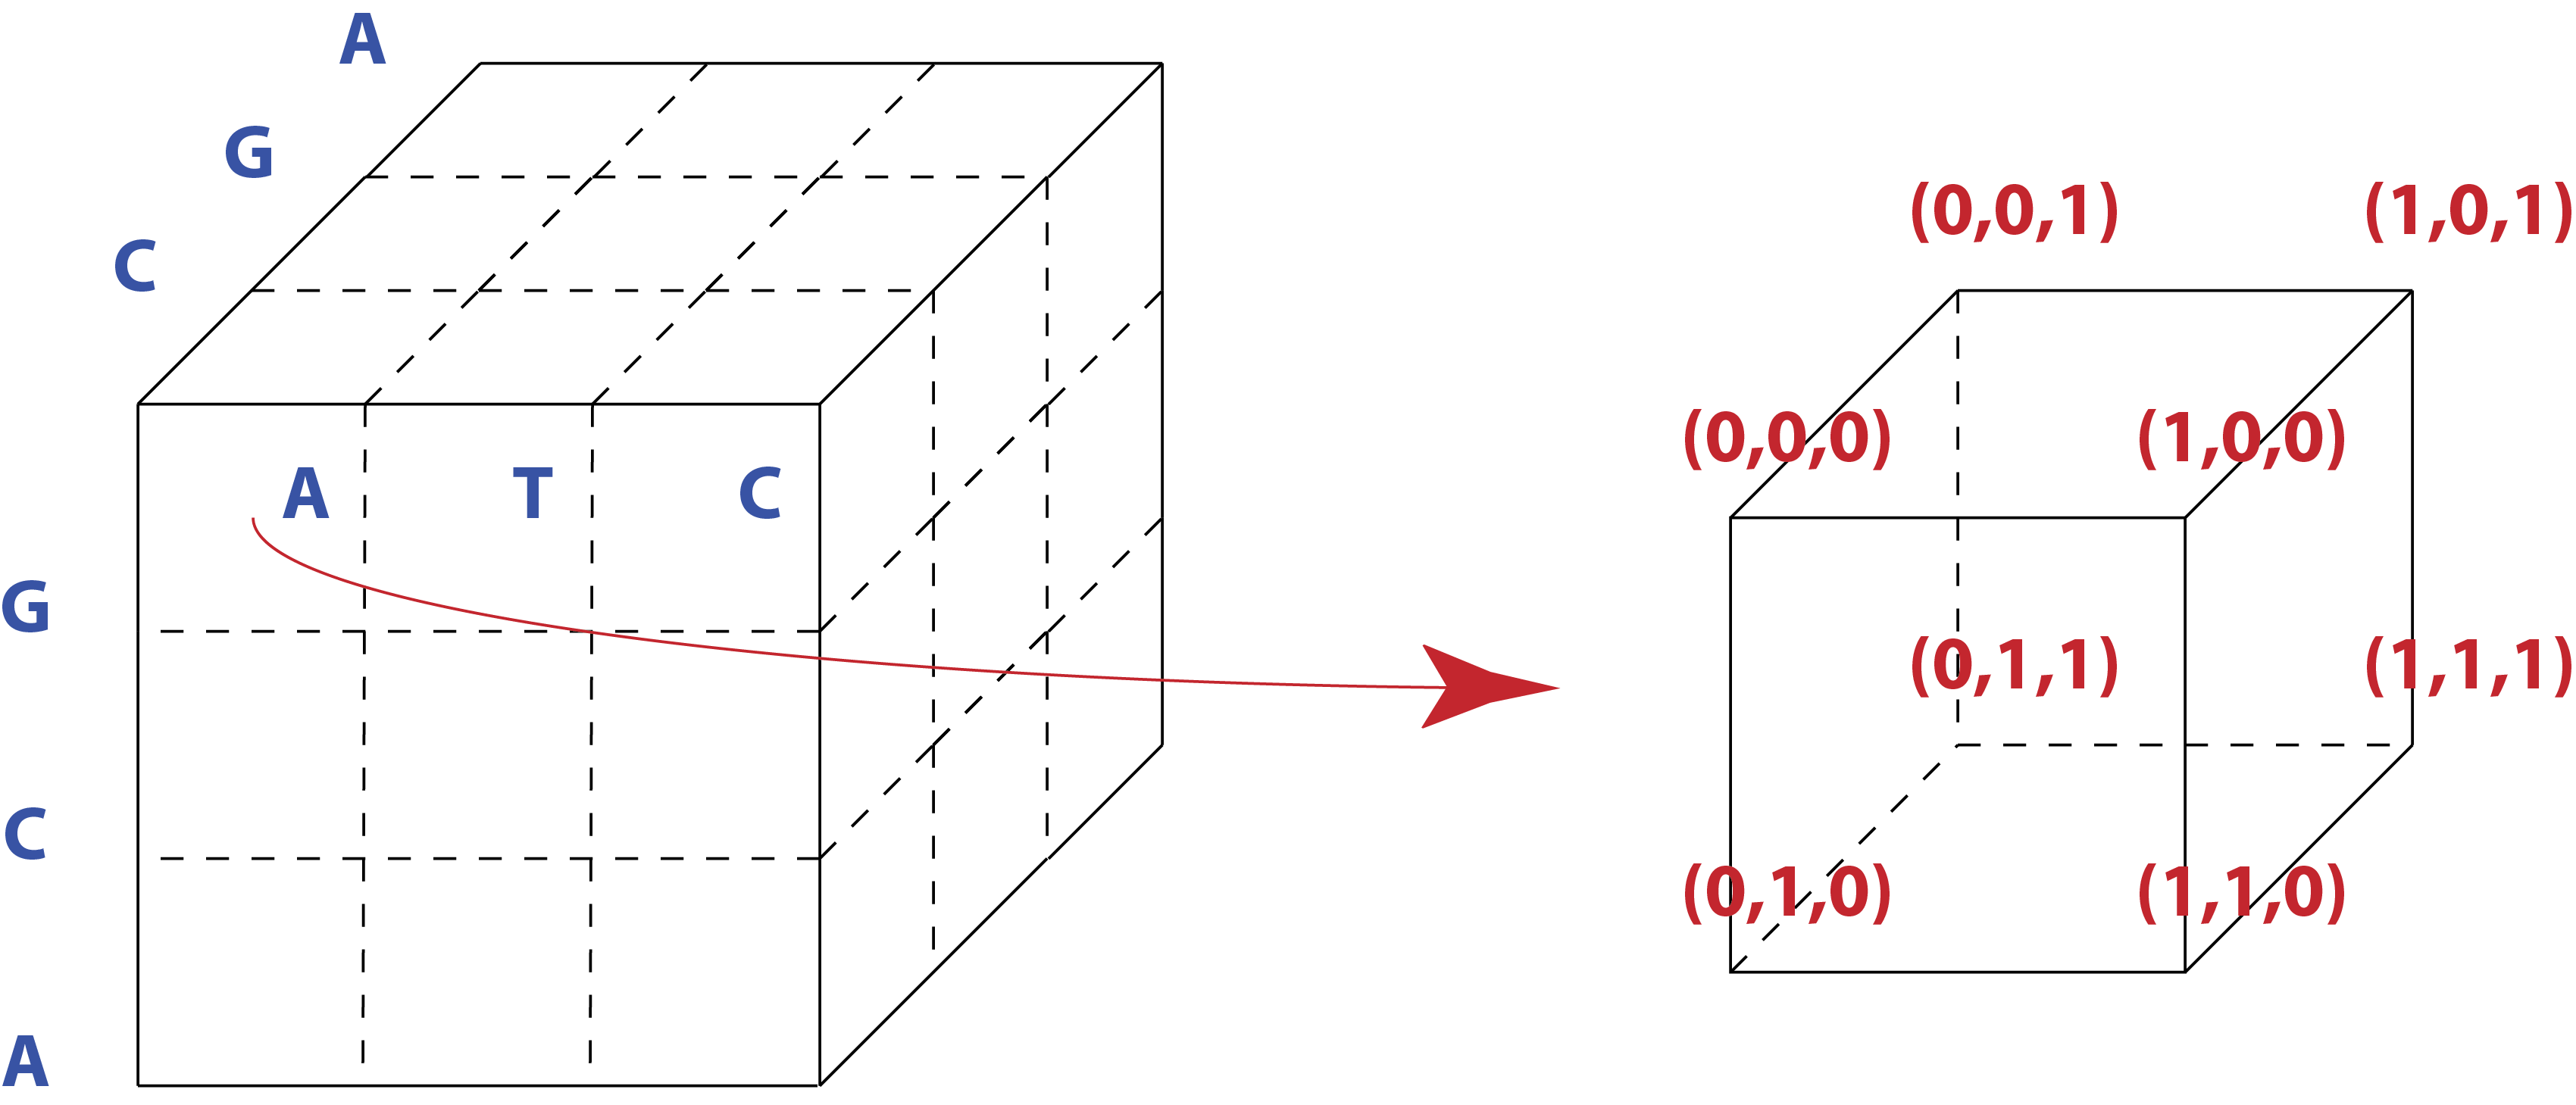
\includegraphics[width=0.5 \textwidth]{fig08/dp_mutiple_dimension.png}
  \caption{A three-dimensional DP array}
\end{figure}

%
% Example of alignment representation
%
\subsubsection*{Example of alignment representation}
\begin{figure}[H]
  \centering
      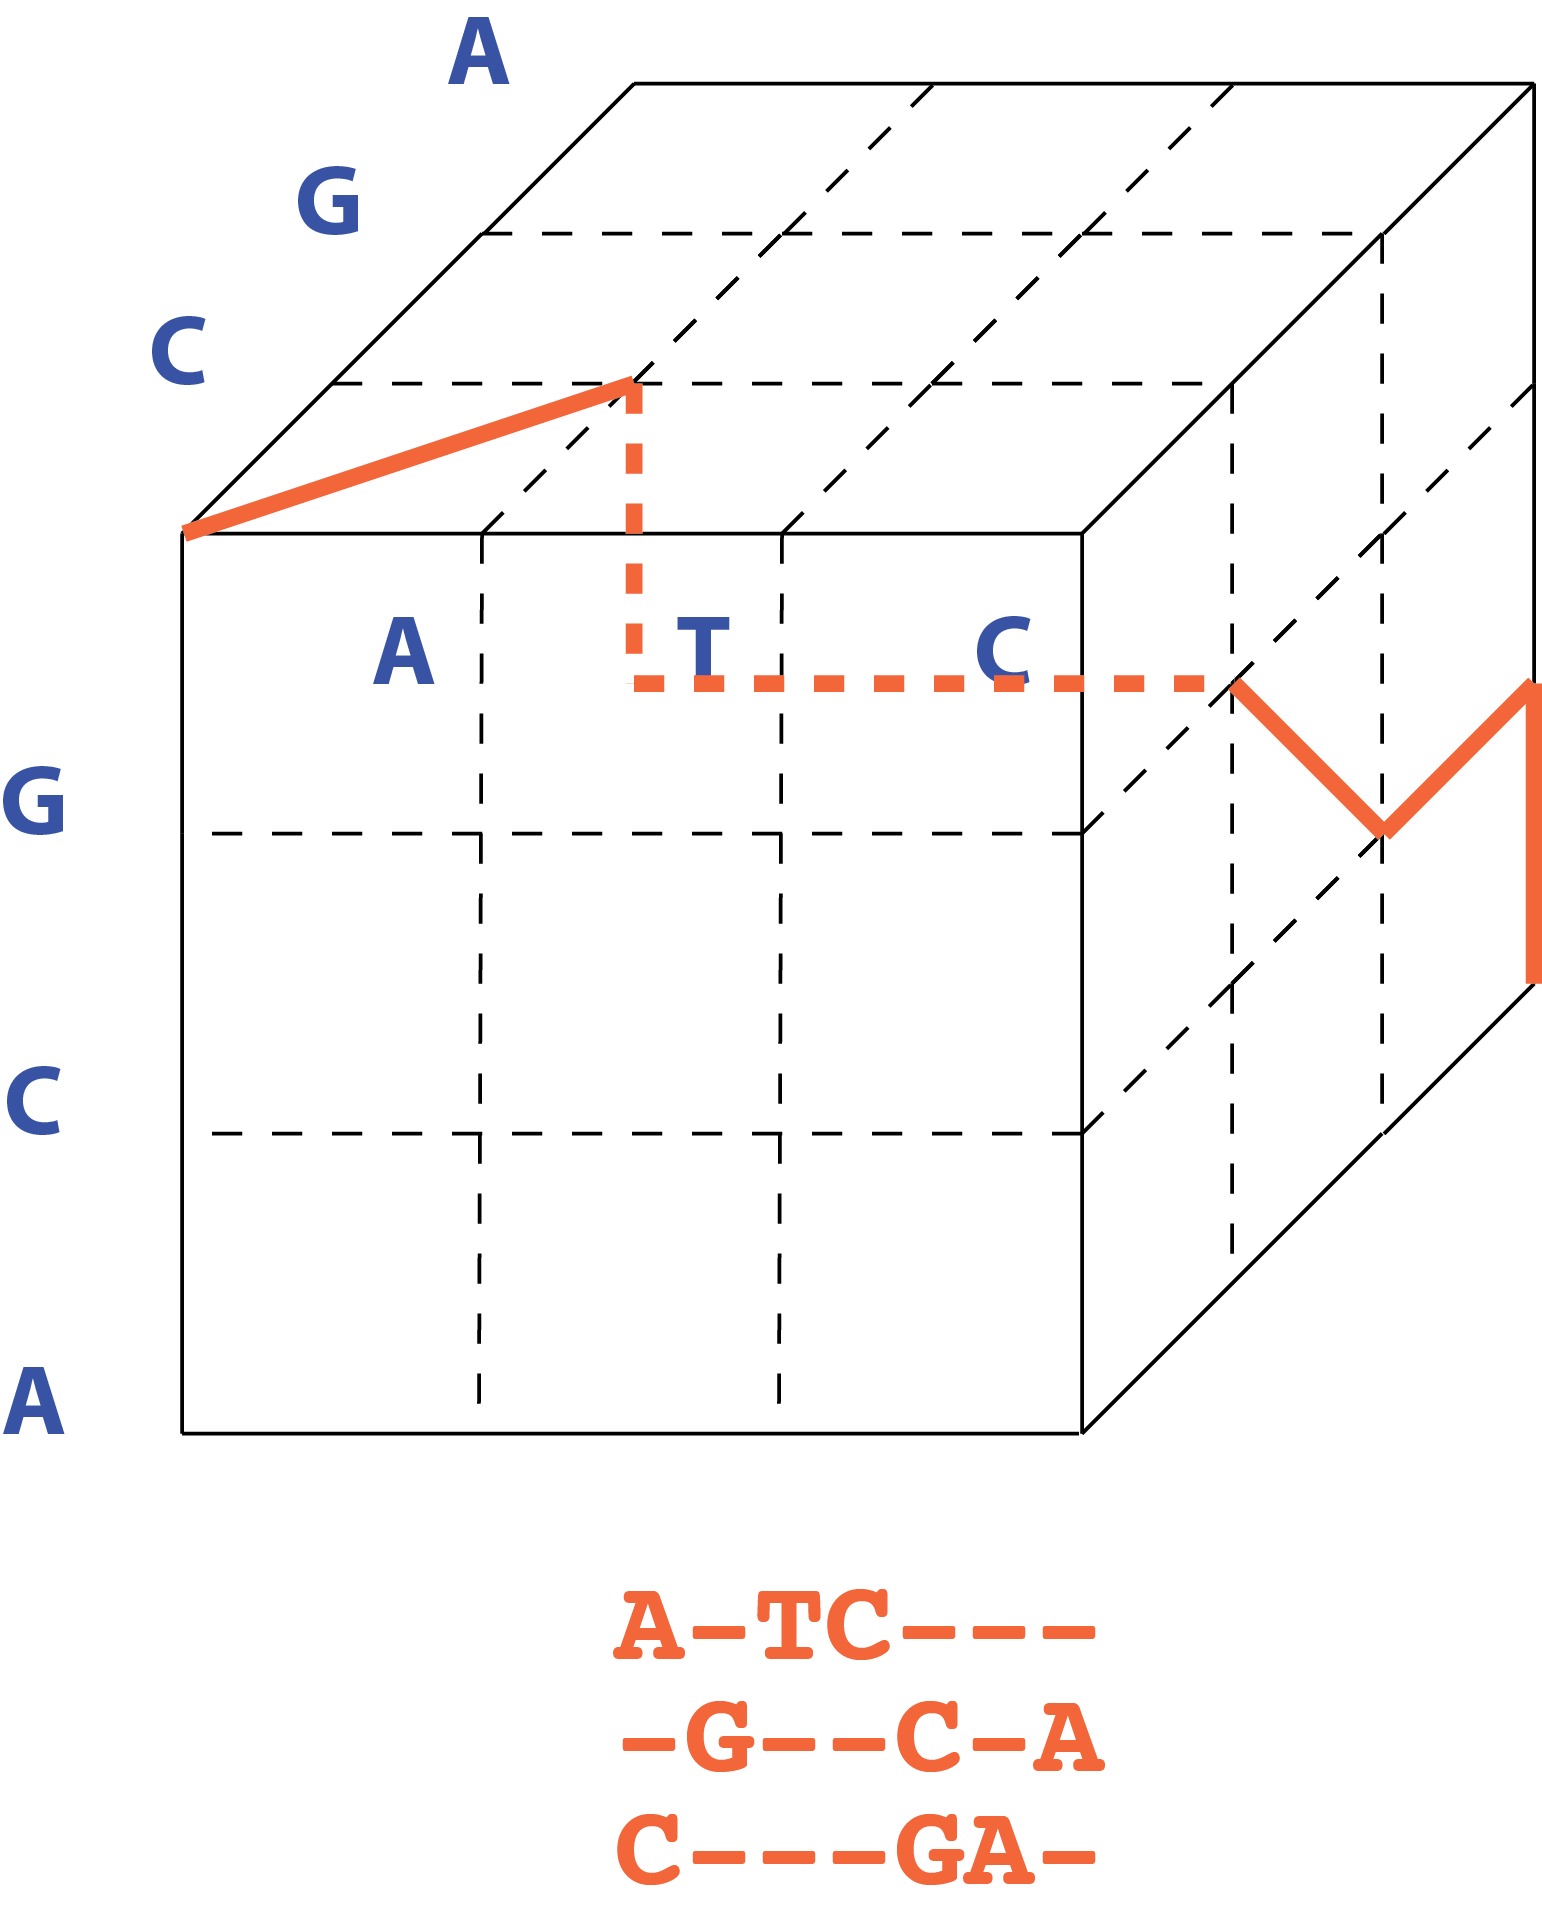
\includegraphics[width=0.2 \textwidth]{fig08/alignment_repsentation.png}
  \caption{An alignment with a three-dimensional DP array}
\end{figure}

%
% The number of candidate scores for a vertex 
%
\subsubsection*{The number of candidate scores for a vertex }
The number of the inbound neighboring vertices is defined as follows. 

\[
\sum_{i=0}^{m-1} \binom{m}{i}  = 2^m - 1
\]

%
% Example of edges of 3-dimensional cell
%
\subsubsection*{Example of edges of 3-dimensional cell}
\begin{figure}[H]
  \centering
      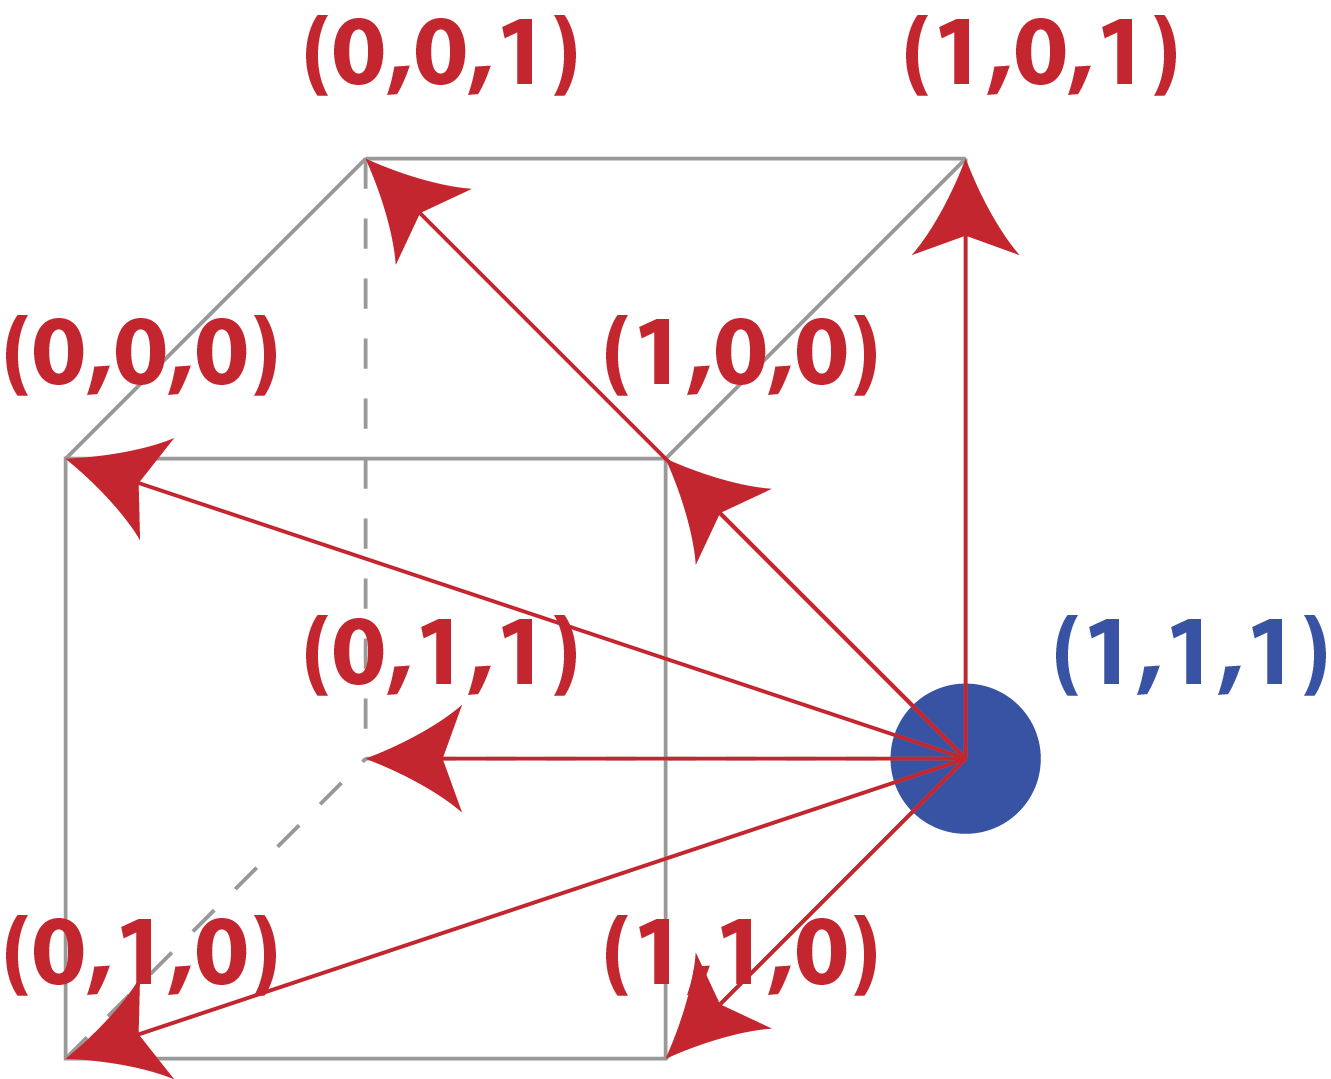
\includegraphics[width=0.25 \textwidth]{fig08/msa_vertex_index.png}
  \caption{An example of seven different edges to one vertex when m = 3}
\end{figure}

%
% A pruning method
%
\subsubsection*{A pruning method}
\begin{itemize}
\item $K$ : a score of an MSA (it does not need to be the optimal)
\item $\nu$ : current vertex
\item $S_{\nu}$ : best score from the start vertex to $\nu$ (by DP)
\item $F_{\nu}$ : best score from the end vertex to $\nu$ (by non-DP)
\item if $S_{\nu}$ + $F_{\nu} < K$ then $\nu$ does not lie on the optimal path
\end{itemize}

\begin{figure}[H]
  \centering
      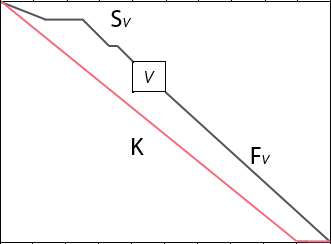
\includegraphics[width=0.3 \textwidth]{fig08/msa_table.png}
  \caption{Score estimation}
\end{figure}

%
% Forward-recursion DP for MSA
%
\subsubsection*{Forward-recursion DP for MSA}
Instead of looking up inbound neighboring vertices, the forward recursion DP sends the calculated score to all outbound neighboring vertices. 

\begin{figure}[H]
  \centering
      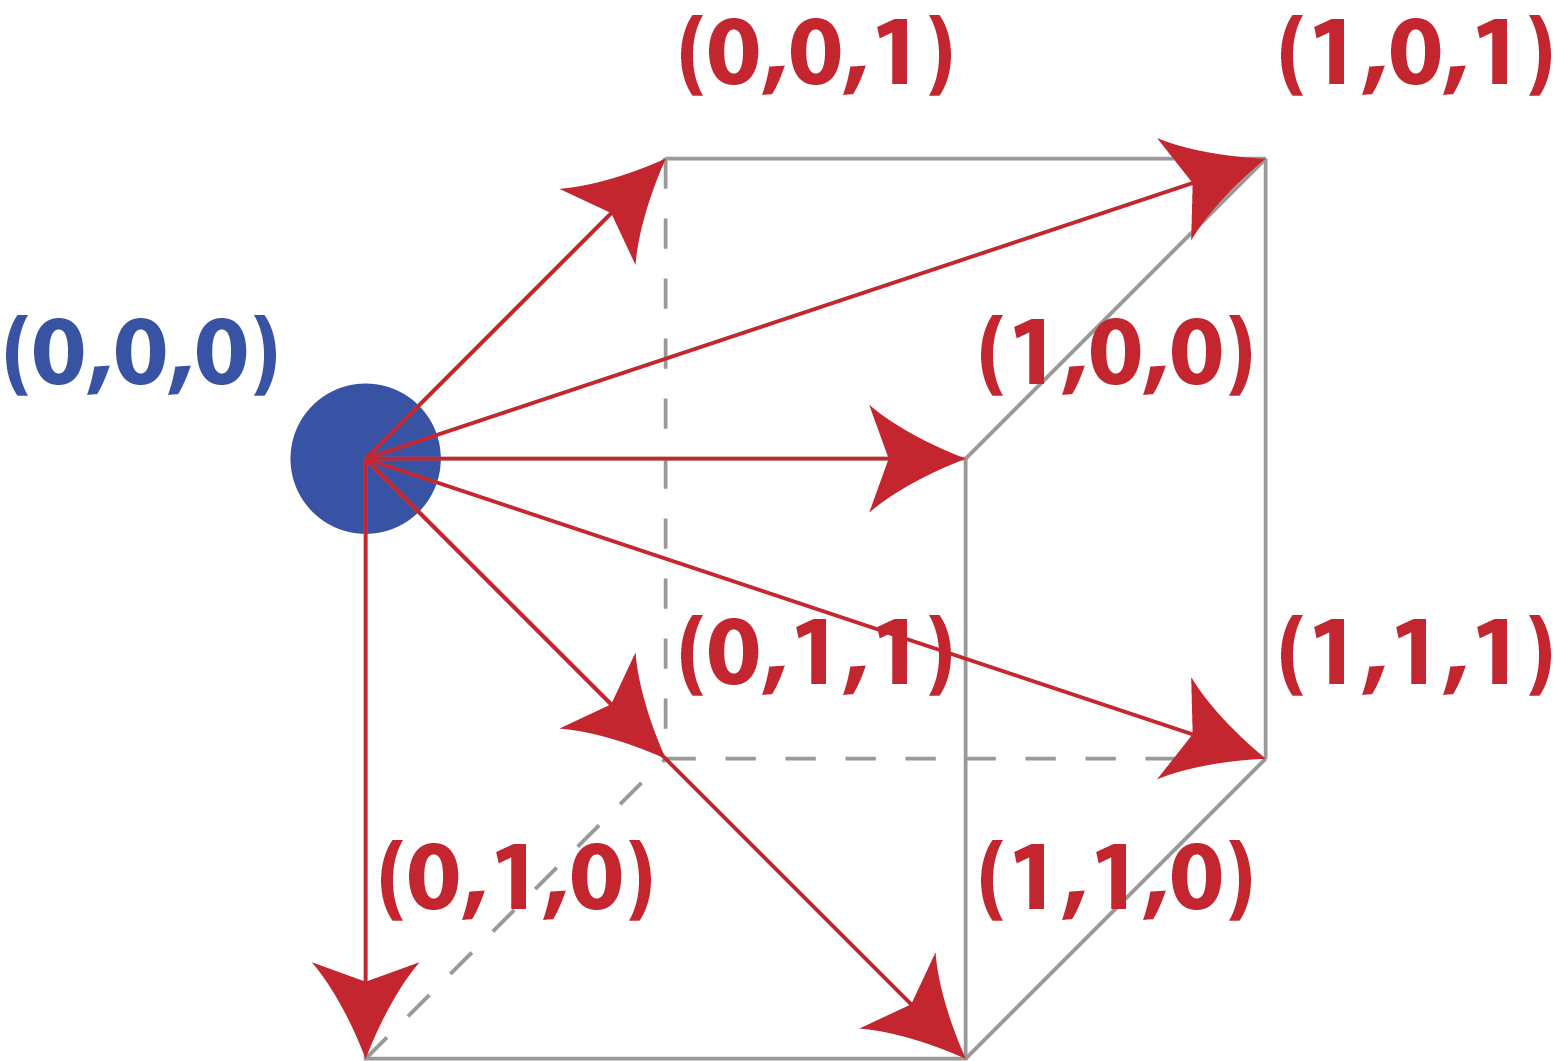
\includegraphics[width=0.3 \textwidth]{fig08/cell_update_msa_feedforward.png}
  \caption{Values are forwarded to all outgoing neighbors}
\end{figure}

\bigskip 

%\end{document}
